% This is LLNCS.DOC the documentation file of
% the LaTeX2e class from Springer-Verlag
% for Lecture Notes in Computer Science, version 2.4
\documentclass{llncs}
\usepackage{cleveref}
\usepackage{llncsdoc}
\usepackage[margin=1in]{geometry}

\begin{document}
\markboth{Independent Study -- Complexity Theory}{Independent Study -- Complexity Theory}
\thispagestyle{empty}

\rule{\textwidth}{1pt}
\vspace{2pt}
\begin{flushright}
\Huge
\begin{tabular}{@{}l}
Independent Study \\ Complexity Theory\\[6pt]
{\large Ryan Dougherty}
\end{tabular}
\end{flushright}
\rule{\textwidth}{1pt}
\vfill

\newpage
\tableofcontents

\newcommand{\classnotation}[1]{\mathcal{#1}}

\newcommand{\dir}{notes}

\section{Introduction \& Preface}

Welcome to this series of lecture notes! The main book that the material comes from is Arora and Barak's \emph{Computational Complexity} book \cite{arora_baraz_computational_complexity}. Some material that is assumed from the reader (and is referenced in \Cref{sec:review}) is from Sipser's \emph{Introduction to the Theory of Computation} book \cite{sipsertheoryofcomp}. We assume that the reader has a reasonable understanding of the following material:
\begin{itemize}
\item \{Regular, Context-free, Turing-decidable, Turing-recognizable\} languages, and their automata counterparts
\item (Un)decidability
\item Reducibility
\item Recursion theorem
\item Time complexity: $\classnotation{P}, \classnotation{NP}, \classnotation{EXPTIME}$, and the -complete versions
\item Space complexity: $\classnotation{PSPACE}, \classnotation{EXPSPACE}, \classnotation{L}, \classnotation{NL}$, and the -complete versions
\end{itemize}
\section{Review}
\label{sec:review}

This section highlights many of the key definitions and theorems studied in a first-year graduate (or advanced undergraduate) course in complexity theory. We assume the reader knows about finite automata (DFAs/NFAs), grammars (CFGs), and Turing machines (TMs), and their respective language classes.

\subsection{(Un)Decidability}

\begin{definition}
A TM is a \emph{decider} if it halts (accepts or rejects) on every input.
\end{definition}

\begin{definition}
A language $B$ is \emph{decidable} if there exists a decider $D$ such that $L(D) = B$. A language $C$ is \emph{undecidable} if $C$ is not decidable.
\end{definition}

\begin{theorem}
The following are decidable:
\begin{itemize}
\item $A_{DFA} = \{\langle M, w \rangle : M$ is a DFA that accepts $w$\}.
\item $E_{DFA} = \{\langle M \rangle : M$ is a DFA whose language is empty\}.
\item $ALL_{DFA} = \{\langle M \rangle : M$ is a DFA whose language is $\Sigma^*$\}.
\item $EQ_{DFA} = \{\langle M_1, M_2 \rangle : M_1$ and $M_2$ are DFAs and $L(M_1) = L(M_2)$\}.
\item $A_{CFG} = \{\langle G, w \rangle : G$ is a CFG that generates $w$\}.
\item $E_{CFG} = \{\langle G \rangle : L(G)$ is empty\}.
\end{itemize}
\end{theorem}

\begin{theorem}
The following are undecidable:
\begin{itemize}
\item $ALL_{CFG} = \{\langle G \rangle : G$ is a CFG and $L(G) = \Sigma^*$\}.
\item $EQ_{CFG} = \{\langle G_1, G_2 \rangle : G_1$ and $G_2$ are CFGs and $L(G_1) = L(G_2)$\}.
\item $A_{TM} = \{\langle M, w \rangle : M$ is a TM that accepts $w$\}.
\end{itemize}
\end{theorem}

\begin{theorem}
The class of decidable languages is closed under complement.
\end{theorem}

\begin{definition}
A language $B$ is \emph{Turing-recognizable} (or recognizable) if there exists a TM that recognizes $B$. A language $C$ is co-Turing-recognizable (or co-recognizable) if it is the complement of some Turing-recognizable language. 
\end{definition}

\begin{theorem}
$A_{TM}$ is not co-recognizable.
\end{theorem}

\begin{theorem}
A language $B$ is decidable if and only if $B$ is recognizable and co-recognizable.
\end{theorem}

\begin{definition}
A function $f: \Sigma^* \rightarrow \Sigma^*$ is a \emph{computable function} if there exists a TM that, on input $w$, halts with $f(w)$ on its tape.
\end{definition}

\subsection{Reducibility}

\begin{definition}
A language $A$ is \emph{mapping-reducible} to language $B$, written $A \le_m B$, if there exists a computable function such that $w \in A$ if and only if $f(w) \in B$.
\end{definition}

\begin{theorem}
If $A \le_m B$ and $B$ is decidable, then $A$ is decidable; if $A$ is undecidable, then $B$ is undecidable.
\end{theorem}

\begin{corollary}
$HALT_{TM} = \{\langle M, w \rangle : M$ is a TM that halts on input $w$\} is undecidable.
\end{corollary}

\begin{definition}
A TM's language has a \emph{property} $P$ (a subset of all TM descriptions) such that whenever $M_1, M_2$ are TMs, and $L(M_1) = L(M_2)$, $\langle M_1 \rangle \in P$ if and only if $\langle M_2 \rangle \in P$. A property $P$ is \emph{nontrivial} if some TM has property $P$ and some other TM does not.
\end{definition}

\spnewtheorem{ricethm}[theorem]{(Rice's Theorem)}{\bfseries}{\itshape}
\begin{ricethm}
Deciding whether a TM has a nontrivial property $P$ of its language is undecidable.
\end{ricethm}

\begin{theorem}
$EQ_{TM} = \{\langle M_1, M_2 \rangle : M_1, M_2$ are TMs and $L(M_1) = L(M_2)$\} is undecidable; also, it is neither recognizable nor co-recognizable.
\end{theorem}

\begin{definition}
A \emph{configuration} of a TM on input $w = w_1\cdots w_n$ in state $q$ is $w_1\cdots w_{i-1}qw_i\cdots w_n$. A \emph{computation history} is a set of configurations delimited by an extra symbol \#: $\#C_1\#C_2\#\cdots\#C_{\ell}\#$, where $C_i$ logically yields $C_{i+1}$. An \emph{accepting computation history} is one such that $C_1$ is the start configuration, and $C_{\ell}$ is an accepting one.
\end{definition}

\begin{definition}
A \emph{linear bounded automaton} (LBA) is a TM that does not allow to move the tape head past the right end of the input.
\end{definition}

\begin{theorem}
$A_{LBA} = \{\langle M, w\rangle : M$ is an LBA that accepts $w$\} is decidable.
\end{theorem}

\begin{definition}
The \emph{Post Correspondence Problem} (PCP) is a puzzle, with a given set of tiles with nonempty ``top strings" and nonempty ``bottom strings." The objective is to list the tiles, repetitions allowed, such that the concatenation of the top strings of all the chosen tiles equals the same of the bottom strings.
\end{definition}

\begin{theorem}
PCP is undecidable.
\end{theorem}

\spnewtheorem{recursionthm}[theorem]{(Recursion Theorem)}{\bfseries}{\itshape}
\begin{recursionthm}
Let a TM $T$ compute a function $t: \Sigma^* \times \Sigma^* \rightarrow \Sigma^*$. Therefore, there exists a TM $R$ that computes a function $r: \Sigma^* \rightarrow \Sigma^*$, such that $r(w) = t(\langle R \rangle, w)$ for all $w$. In other words, every TM can obtain their own description.
\end{recursionthm}

\begin{definition}
A TM $M$ is \emph{minimal} if there does not exist a TM $N$ that has fewer states and $L(M) = L(N)$.
\end{definition}

\begin{theorem}
$MIN_{TM} = \{\langle M \rangle : M$ is a TM and is minimal\} is not recognizable.
\end{theorem}


\section{Polynomial Hierarchy, Alternating TMs}

From \Cref{thm:relativizePandNP}, we have a notion of using {\P} and {\NP} with the power of oracle machines. However, we don't have a generalization of a ``hierarchy" of such oracle machines (the theorem only concerns the ``first level"). Therefore, in \cite{originalpolyhierarchypaper}, the notion of a ``polynomial hierarchy" was created. The hierarchy is defined (equivalently) as follows:
\begin{itemize}
\item $\Delta_0^\P = \Sigma_0^\text{\P}$ = $\Pi_0^\text{\P} = \text{\P}$,
\item $\Delta_i^\text{\P} = \text{\P}^{\Sigma_{i-1}^\text{\P}}$, 
\item $\Sigma_i^\text{\P} = \text{\NP}^{\Sigma_{i-1}^\text{\P}}$, 
\item $\Pi_i^\text{\P} = \text{\coNP}^{\Sigma_{i-1}^\text{\P}}$.
\end{itemize}

\begin{figure}
\label{fig:polyhierarchy}
\centering
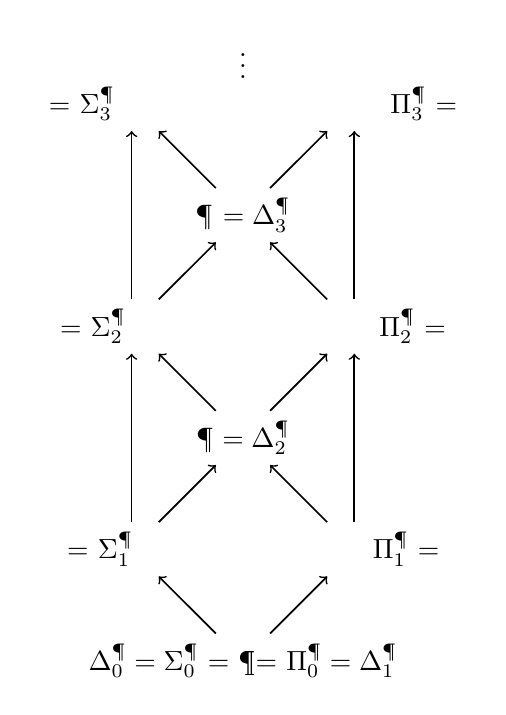
\begin{tikzpicture}[->, node distance=2cm, semithick]
 \node (P) {$\Delta_0^\P = \Sigma_0^\P$ = \P = $\Pi_0^\text{\P} = \Delta_1^\text{\P}$};
 \node (Sigma1) [above left of=P]       {{\NP} = $\Sigma_1^\text{\P}$ \hspace*{0.8cm}};
 \node (Pi1)    [above right of=P]      {\hspace*{1.2cm} $\Pi_1^\text{\P}$ = \coNP};
 \node (Delta2) [above left of=Pi1]     {$\text{\P}^\text{\NP} = \Delta_2^\text{\P}$ };
 \node (Sigma2) [above left of=Delta2]  {$\text{\NP}^\text{\NP}$ = $\Sigma_2^\text{\P}$ \hspace*{1.0cm}};
 \node (Pi2)    [above right of=Delta2] {\hspace*{1.5cm} $\Pi_2^\text{\P}$ = $\text{\coNP}^\text{\NP}$};
 \node (Delta3) [above left of=Pi2]     {$\text{\P}^{\text{\NP}^\text{\NP}} = \Delta_3^\text{\P}$};
 \node (Sigma3) [above left of=Delta3]  {$\text{\NP}^{\text{\NP}^\text{\NP}}$ = $\Sigma_3^\text{\P}$ \hspace*{1.3cm}};
 \node (Pi3)    [above right of=Delta3] {\hspace*{1.8cm} $\Pi_3^\text{\P}$ = $\text{\coNP}^{\text{\NP}^\text{\NP}}$};
 \node (dots)   [above of=Delta3]       {\vdots};
 \draw (P)      -> (Sigma1);
 \draw (P)      -> (Pi1);
 \draw (Sigma1) -> (Sigma2);
 \draw (Sigma1) -> (Delta2);
 \draw (Pi1)    -> (Pi2);
 \draw (Pi1)    -> (Delta2);
 \draw (Delta2) -> (Sigma2);
 \draw (Delta2) -> (Pi2);
 \draw (Sigma2) -> (Sigma3);
 \draw (Sigma2) -> (Delta3);
 \draw (Pi2)    -> (Pi3);
 \draw (Pi2)    -> (Delta3);
 \draw (Delta3) -> (Sigma3);
 \draw (Delta3) -> (Pi3);
\end{tikzpicture}
\caption{Polynomial Hierarchy, taken from http://commons.wikimedia.org/wiki/File:Polynomial\_time\_hierarchy.svg. Each arrow represents inclusion: for example, $\Sigma_1^\text{\P} \subseteq \Delta_2^\text{\P} \subseteq \Sigma_2^\text{\P}$.}
\end{figure}

\begin{definition}
The \emph{polynomial hierarchy}, called \PH, is defined to be:
\[
\text{\PH} = \bigcup_{k = 1}^{\infty} \Sigma_k^{\text{\P}}
\]
\end{definition}

For {\PH}, we often call the $i$-th level of {\PH} to be both $\Sigma_i^\text{\P}$ and $\Pi_i^\text{\P}$. A natural inclination, as has been done before with \NP, \PSPACE, \NL, and the like, is to find a complete problem for {\PH}. However, the following theorem shows that this is most likely not the case.

\begin{theorem}
If there is a \PH-complete language, then {\PH} only has a finite number of levels.
\end{theorem}

\begin{proof}
Assume there exists a \PH-complete language, and let it be $L$. By definition, $\text{\PH} = \bigcup_{k = 1}^{\infty} \Sigma_k^{\text{\P}}$. Therefore, for some $j$, we have that $L \in \Sigma_j^\P$, and every language in {\PH} is polynomial-time reducible to $L$. However, any language $A$ that is polynomial-time reducible to some language $B \in \Sigma_j^\P$ has that $A \in \Sigma_j^\P$. Therefore, $\PH \subseteq \Sigma_j^\P$.
\end{proof}
\section{Boolean Circuits}

We have looked a little at boolean formulas, which take input variables that have values ``true" or ``false" and, through some operations, give a result of either ``true" or ``false" as ``output." Here, we look at circuits, which are a generalization of formulas.

\begin{definition}
A \emph{boolean circuit} is a DAG (directed acyclic graph) with a number of ``source" vertices (those with no incoming edges), also called ``gates," and a ``sink" vertex (with no outgoing edges), also called the ``output." Vertices are labelled with $\wedge, \vee, \neg$ - those with $\wedge, \vee$ have fan-in 2 and fan-out 1, and those with $\neg$ have fan-in and fan-out 1. The \emph{size} of a circuit is the number of vertices it has. The output of a particular input $x \in \{0, 1\}^n$ is applying each of the vertex ``rules" recursively until the output is reached. 
\end{definition}

\begin{theorem}
Any circuit with its $\wedge, \vee$ vertices having bounded fan-in (i.e., $\ge 3$) can be converted to an equivalent circuit with these vertices having only fan-in 2. 
\end{theorem}

\begin{definition}
A \emph{$T(n)$-size circuit family} is a sequence of circuits (i.e., $\{C_n\}_{n \in \mathbb{N}}$), where, for a given function $T \colon \mathbb{N} \rightarrow \mathbb{N}$, has that all of the circuits have size $\le T(n)$ for all $n$. We say that $L \in \SIZE(T(n))$ if there exists a $T(n)$-size circuit family such that for all $x \in \{0, 1\}^n$, $x \in L$ if and only if $C_n(x) = 1$ (i.e., ``accepts" $x$). 
\end{definition}

We start with an example: $L_1 = \{1^n \colon n \in \mathbb{Z}\}$.
\begin{theorem}
\label{thm:unary_linear_circuit_family}
$L_1$ can be decided by a linear-sized circuit family. 
\end{theorem}

\begin{proof}
The circuit is simply a tree of $\wedge$ gates that computes that of all inputs. 
\end{proof}

\begin{definition}
We define $\Ppoly$ to be $\bigcup_{c} \SIZE(n^c)$; in other words, $\Ppoly$ is the set of languages with poly-size circuit families.
\end{definition}

\begin{theorem}
\label{thm:all_unary_ppoly}
All unary languages are in $\Ppoly$.
\end{theorem}

\begin{proof}
Implied by \Cref{thm:unary_linear_circuit_family}.
\end{proof}

\begin{theorem}
\label{thm:p_subset_ppoly}
$\P \subseteq \Ppoly$, and the inclusion is strict.
\end{theorem}

\begin{proof}
Let $M$ be an ``oblivious" TM, which is one that has its head movement independent of the input. We need to show that for any $T(n)$-time oblivious TM, we can construct an equivalent $O(T(n))$-size circuit family. 

\par Let $x$ be an input for $M$, and look at the set of $M$'s configurations: $C_1, \cdots, C_{T(n)}$. Encode each configuration by a constant-size binary string. We can compute $C_i$ based on the following:
\begin{itemize}
\item $x$ itself,
\item $C_{i-1}$,
\item $C_{i_1}, \cdots, C_{i_k}$, where $C_{i_j}$ is the last step that $M$'s $j$th head was in the same position as it is in the $i$th step.
\end{itemize}
Because we assumed $M$ is oblivious, then $i_1, \cdots, i_k$ does not depend on $x$ - they only depend on $i$. Therefore, since we only have a constant number of strings of constant size, we can compute $C_i$ with a constant-size circuit.

\par We compose these circuits together so that, on input $x$, we compute $C_{T(n)}$ on $M$'s last step in its execution on $x$. We also have a constant size circuit that outputs 1 if and only if $C_{T(n)}$ is an accepting configuration. Since we have $O(T(n))$ circuits of constant size, we have constructed an equivalent $O(T(n))$-size circuit to $M$.

\par For showing strict containment, by \Cref{thm:all_unary_ppoly}, all undecidable unary languages are in $\Ppoly$, which are by definition not in $\P$.
\end{proof}



\newcommand{\CKTSAT}{\lang{CKT-SAT}}
\subsection{\CKTSAT}
As we proved the Cook-Levin Theorem from before, now we prove the circuit analog of $\SAT$. $\CKTSAT$ is the set of all circuits that have a ``satisfying assignment" to the $n$ input variables. In other words, there exists a $w \in \{0, 1\}^n$ if and only if $C(w)=1$ if $C \in \CKTSAT$.

\begin{theorem}
$\CKTSAT$ is $\NP$-complete.
\end{theorem}

\begin{proof}
$\CKTSAT$ is clearly in $\NP$. For hardness, if $L \in \NP$, then there is a verifier $V$ such that, on input $x$, verifies if $x \in L$ in polynomial time. By \Cref{thm:p_subset_ppoly}, we can convert $V$ into an equivalent circuit $C$ in polynomial time. Therefore, $x \in L$ if and only if $C \in \CKTSAT$.
\end{proof}

\subsection{Advice!}
We defined $\Ppoly$ in one way - now we will see another. This will make the fact that all undecidable unary languages are in $\Ppoly$ to be more clear. 

\begin{definition}
The set of languages \emph{decidable by $T(n)$-time TMs with $A(n)$ bits of advice} is called $\DTIME(T(n))/A(n)$. By this, we mean that for every $L \in \DTIME(T(n))/A(n)$, there is a sequence of strings, $\{a_n\}$, each of length $A(n)$, and a $T(n)$-time verifier $M$, such that it accepts $\langle x, a_n \rangle$ if and only if $x \in L$.
\end{definition}

In other words, we are given a sequence of strings of length $A(n)$ that are certificates, in a sense. Now we will look at the alternative definition of $\Ppoly$:
\begin{theorem}
$\Ppoly$ can be re-defined to be $\bigcup_{c, d \ge 0} \DTIME(n^c)/n^d$.
\end{theorem}

\begin{proof}
By the first definition of $\Ppoly$, if $L \in \Ppoly$, then $L$ is computable by a poly-size circuit family $\{C_n\}$. We can just use the descriptions of each of the $C_n$ as an advice string, and the TM is poly-time that, on input $\langle x, C \rangle$, where $C$ is an $n$-input circuit, outputs $C(x)$. 

\par If $L$ is decided by a poly-time TM $M$ with access to the sequence of advice strings $\{a_n\}$, each of poly-length, then we can use the construction of \Cref{thm:p_subset_ppoly} to obtain an equivalent poly-size circuit $B_n$ for all $n$ (i.e., outputs the same as $M$ does). Let $C_n$ be the same as $B_n$ but with $a_n$ hard-coded as the second input (i.e., fix the inputs). Therefore, $\{C_n\}$ is the desired circuit-family.
\end{proof}

We can actually get a ``nondeterministic" parallel to \Cref{thm:p_subset_ppoly}:

\begin{theorem}
$\NP \subseteq \bigcup_{c, d \ge 0} \NTIME(n^c)/n^d$, and the inclusion is strict (note $\NTIME$ instead of $\DTIME$).
\end{theorem}

\begin{proof}
It's easy to see inclusion: set $d = 0$, and have an $\NP$ machine accept a one-bit advice string for every $n$, and have the machine ignore the advice. 

\par For strict inclusion, we know that all unary languages are in $\DTIME(n)/1 \subseteq \NTIME(n)/1$, because we only need one bit of advice for each $n$ in advising the machine to check if $1^n$ is in the language. However, the following undecidable language is also in there, and therefore is not in $\NP$:
\begin{center}
$UHALT = \{1^n \colon n$'s binary expansion encodes $\langle M, w \rangle$ where $M$ halts on $w$\}.
\end{center}
\end{proof}

We have proved both of these, but how does $\NP$ relate to $\Ppoly$ (instead of the $\NTIME$ version)? We actually don't know for sure, as the polynomial hierarchy would collapse:

\begin{theorem}[Karp-Lipton]
If $\NP \subseteq \Ppoly$, then $\PH = \Sigma_2^\P$.
\end{theorem}

\begin{proof}
It is sufficient to show that $\NP \subseteq \Ppoly$ implies $\Sigma_3^\P \subseteq \Sigma_2^\P$. So fix a language $L \in \Sigma_3^\P$. By definition, there exists a poly-time TM $M$ and a polynomial $p$ such that if $x \in L$, then:
\begin{center}
$\exists u_1 \in \{0, 1\}^{p(|x|)} \forall u_2 \in \{0, 1\}^{p(|x|)} \exists u_3 \in \{0, 1\}^{p(|x|)} M(x, u_1, u_2, u_3)$ accepts.
\end{center}
We re-arrange this as follows with a new language $L'$: $\langle x, u_1, u_2 \rangle \in L'$ if and only if:
\begin{center}
$\exists u_3 \in \{0, 1\}^{p(|x|)} M(x, u_1, u_2, u_3)$ accepts.
\end{center}
Therefore, $L' \in \NP$ and therefore $L' \le_P \ThreeSAT$. Therefore, $\langle x, u_1, u_2 \rangle \in L'$ if and only if there exists a $\ThreeSAT$ formula $\phi$ over $x, u_1, u_2$ (reduction done in poly time). Also a NDTM $M'$ decides $L'$.

\par Now just plug in $M'$: $x \in L$ if and only if:
\begin{center}
$\exists u_1 \in \{0, 1\}^{p(|x|)} \forall u_2 \in \{0, 1\}^{p(|x|)} M'(x, u_1, u_2)$ accepts.
\end{center}
This is equivalent to:
\begin{center}
$\exists u_1 \in \{0, 1\}^{p(|x|)} \forall u_2 \in \{0, 1\}^{p(|x|)} \phi(x, u_1, u_2) \in \ThreeSAT$.
\end{center}
Now here is the central part of the proof. We assume that $\NP \subseteq \Ppoly$. Therefore, there exists a poly-size circuit $C$ for $\ThreeSAT$. We can just use $C$ to decide the expression above. So how do we find the circuit in the first place?

\par We prove the following. There exists a poly-time TM $M_C$ that, on input 3CNF formula $\phi$ with $|\phi| = n$ and a circuit $C$ with $n$ inputs such that: 
\begin{enumerate}
\item If $C$ recognizes $\ThreeSAT$ for inputs of length $n$ and $\phi \in \ThreeSAT$, then $M_C$ accepts.
\item If $\phi \notin \ThreeSAT$, then $M_C$ rejects.
\end{enumerate}
The idea is the following: repeatedly use the circuit $C$ to extract a satisfying assignment for $\phi$. Let the variables of $\phi$ be $x_1, ..., x_k$. If $C$ on input $\phi$ outputs 0, then $M_C$ rejects. Otherwise, fix $x_1$ to be false, and check if $C$ outputs 1 on the new circuit. If so, permanently fix $x_1$ to be false, and also have an array of $k$ values, and store $x_1$ to be the first element. Repeat for the other $k-1$ variables. Now we check: if $\phi$ with the assignments given have $\phi$ be true, then accept; otherwise, reject.

\par So now we go back to the original proof: we modify the statement above to be:
\begin{center}
$\exists C$ of poly-size $\exists u_1 \in \{0, 1\}^{p(|x|)} \forall u_2 \in \{0, 1\}^{p(|x|)} \M_C(C, \langle x, u_1, u_2\rangle)$ accepts.
\end{center}
Therefore, $L \in \Sigma_2^\P$.
\end{proof}

\subsection{$\AC, \NC$}
We have dealt with circuits of polynomial size, but what about the other direction? We define a similar analogue of $\L, \NL$ in space complexity but for circuits.

\begin{definition}
For $d \in \mathbb{N}$, we say $L \in \NC^d$ if L is decided by a family of poly-size, $O(\log^d n)$-depth circuits $\{C_n\}$, and $L \in \AC^d$ the same way but the gates have unbounded fan-in. We also define $\NC = \bigcup_{d \ge 0}\NC^d$ and $\AC = \bigcup_{d \ge 0}\AC^d$.
\end{definition}
So how much power does unbounded fan-in give? It only gives enough power to add a log-factor:

\begin{theorem}
$\NC^d \subseteq \AC^d \subseteq \NC^{d+1}$.
\end{theorem}
\begin{proof}
Unbounded fan-in can be simulated by a $O(\log n)$-depth tree of OR/AND gates.
\end{proof}

We also show that it is unlikely that any finite level of the $\NC^d$ hierarchy collapses (just like the $\PH$ hierarchy):
\begin{theorem}
$\NC^d = \NC^{d+1} \Rightarrow \NC = \NC^i$.
\end{theorem}

\begin{proof}
We show that $\NC^d = \NC^{d+1}$ implies $\NC^{d+1} = \NC^{d+2}$, from which the result follows. For a circuit $C$ of depth $O(\log^{d+2} n)$, partition it into $O(\log n)$ layers of size $O(\log^{d+1} n)$ each. Each partition $j$'s output is the input of $j+1$, and each contains polynomially many bits. Each bit at partition $j+1$ is computed from $j$ by a $\NC^{d+1}$ circuit. Since $\NC^d = \NC^{d+1}$, replace it by a $\NC^d$ circuit (may not be the same size, but can only be polynomially larger). This replacement has a circuit of poly-size, depth $O(\log^{d+1} n)$, and fan-in 2. Therefore, $\NC^{d+2} = \NC^{d+1} = \NC^d$. 
\end{proof}
Therefore, it is most likely that each inclusion of $\NC^d \subseteq \AC^d \subseteq \NC^{d+1}$ is strict (except for $d = 0$). 

\subsection*{Exercises}

\begin{enumerate}
\item A language $L \subseteq \{0, 1\}^*$ is sparse if there is a polynomial $p$ such that $|L \cap \{0, 1\}^n| \le p(n)$ for every $n \in \mathbb{N}$. Show that every sparse language is in $\Ppoly$.
\item Going off the previous question, show that if a sparse language is $\NP$-complete, then $\P = \NP$.
\end{enumerate}
\section{Randomization}

In the previous sections, we have only dealt with (non)-deterministic TMs. However, there are many important classes that relate a TM when using a probability, as we define below:

\begin{definition}
A \emph{probabilistic TM} (PTM) has two transition functions, and at each step we choose, independently with probability $\frac{1}{2}$, to apply one of the two functions, like a coin flip. We say that a PTM $M$ halts in $T(n)$ time if $M$ halts on all inputs $x$ within $T(|x|)$ steps, regardless of the choices made during execution.
\end{definition}

We can now define the probabilistic analog of $\P$, which is $\BPP$:
\begin{definition}
A language $L$ is in $\BPTIME(T(n))$ if there exists a PTM $M$ that decides $L$ in time $T(n)$, $M$ halts within $T(|x|)$ steps regardless of choices, and $\Pr[M(x) = L(x)] \ge \frac{2}{3}$, where $L(x) = 1$ if $x \in L$, and $L(x) = 0$ if $x \notin L$. We define:
\[
\BPP = \bigcup_{c \ge 0}\BPTIME(n^c)
\]
\end{definition}

It is clear that $\P \subseteq \BPP$: the definition of $\P$ is the same except without coin flips, and has zero error in accepting/rejecting probability. We also give an alternate definition for $\BPP$:
\begin{definition}
$L \in \BPP$ if there exists a poly-time TM verifier $M$ and a polynomial $p$ such that for all $x \in \{0, 1\}^*$, $\Pr[L(M) = L] \ge \frac{2}{3}$ where $M$ has certificates of size $p(|x|)$.
\end{definition}

\begin{theorem}
$\BPP \subseteq \Ppoly$.
\end{theorem}

This proof will use what is called ``success amplification" - the essential idea is that, given we have polynomial time, we can make successive coin flips to reduce the error bound for $\BPP$ to even less error. We do this as follows:
\begin{itemize}
\item For a PTM $M$ that computes a language $L$ with error $\frac{1}{2} - \frac{1}{n^c}$, run $M$ for $k$ independent trials, and accept only if at least half of the trials accept. 
\item Define $X_i = 1$ if the $i$-th trial accepts, and 0 otherwise, and $X = \Sigma_1^k X_i$. 
\item Therefore, $\Pr[X_i = 1] \ge \frac{1}{2} + \frac{1}{n^c}$. Call this result $p$.
\item $\E[X] \ge pk$ for the same reasoning.
\item Call $\delta = 1-\frac{1}{2p}$.
\end{itemize}
Therefore, now we want to find the probability that the trials done above are incorrect, by using Chernoff bounds:
\begin{center}
$\Pr[X < (1-\delta)pk] \le \exp(\frac{-{(1-\frac{1}{2p})^2}pk}{2}) \le \exp(-\frac{k}{2n^{2c}})$
\end{center}
So, for $k$ a polynomial (i.e., $2n^{2c+d}$), we can have an exponentially small error bound. Now, onto the proof.

\begin{proof}
Let $L \in \BPP$. By success amplification, there is a poly-time TM $M$ such that $L(M) = L$ with error smaller than $2^{-n}$. Choose an $x \in \{0, 1\}^n$. Therefore, $\Pr[\text{$M$ computes incorrectly on $x$}] < \frac{1}{2^n}$. We can observe that:
\[
\Pr[\text{$M$ computes incorrectly on some $y \in \{0, 1\}^n$}] \le \Sigma_{x \in \{0, 1\}^n} \Pr[\text{$M$ computes incorrectly on $x$}] = 1
\]
Therefore, there are some coin flips where $M$ does not make any error on any $x \in \{0, 1\}^n$. All we need to do is convert $M$ into a circuit and hardwire these coin flips, which completes the proof. 
\end{proof}

\begin{theorem}[Sipser-G\'{a}cs]
$\BPP \subseteq \Sigma_2^\P \cap \Pi_2^\P$.
\end{theorem}

\begin{proof}
As before, assume that for an $L \in \BPP$ there is a poly-time TM $M$ such that $L(M) = L$ with error smaller than $2^{-n}$. Since $\BPP$ is closed under complement, we only need to show $\BPP \subseteq \Sigma_2^\P$.

\par For $x \in \{0, 1\}^n$, let $S_x$ be the set of certificates for which $M$ accepts $x$, and let $p$ be the polynomial that is the number of random bits $M$ uses. Therefore, either $|S_x| \ge (1-2^{-n})2^{p(n)}$, or $|S_x| \le 2^{p(n)-n}$, whether $x \in L$ or not. What we will show is that we can differentiate between these using only 2 quantifiers.

\par For $A \subseteq \{0, 1\}^{p(n)}$ and $b \in \{0, 1\}^{p(n)}$, define $A+b = \{a+b \colon a \in A\}$, where the operation is done $\mod 2$. Let $k = \lceil {p(n)/n} \rceil +1$. We will show the following:

\begin{enumerate}
\item For all $S \subseteq \{0, 1\}^{p(n)}$ and $|S| \le 2^{p(n)-n}$ and any $k$ vectors $\{u_i\}_{1 \le i \le k}$ with $u_i \in \{0, 1\}^{p(n)}$, we have that $\bigcup_{i=1}^{k} (S+u_i) \ne \{0, 1\}^{p(n)}$ (i.e., if $|S|$ is ``small," then we cannot get all of $\{0, 1\}^{p(n)}$). 

\item For all $S \subseteq \{0, 1\}^{p(n)}$ and $|S| \ge (1-2^{-n})2^{p(n)}$, there exist $k$ vectors $\{u_i\}_{1 \le i \le k}$ with $\bigcup_{i=1}^{k}(S+u_i) = \{0, 1\}^{p(n)}$ (i.e., if $|S|$ is ``large," then we can get all of $\{0, 1\}^{p(n)}$).
\end{enumerate}
In other words, we can establish that $x \in L$ with only 2 quantifiers. Proving these implies that $\BPP \subseteq \Sigma_2^\P \cap \Pi_2^\P$. For the first proof, we have that $|S + u_i| = |S|$, so the union is at most $k|S| < 2^{p(n)}$ for large enough $n$.

\par For the second proof, if the $u_i$ are chosen independently randomly, then $\Pr[\bigcup_{i=1}^{k}(S+u_i) = \{0, 1\}^{p(n)}] > 0$ will imply the proof. Let $B_r$ be the event that $r \notin \bigcup_{i=1}^{k}(S+u_i)$. This implies that we need to prove that $\Pr[\exists B_r] < 1$ for some $r \in \{0, 1\}^{p(n)}$. Equivalently, we can show that $\Pr[B_r] < 2^{-p(n)}$ for all $r$. 

\par Define $B_r^i$ the event that $r \notin S + u_i$ (equivalently, $r + u_i \notin S$). We can see that $B_r = \bigcap_{1 \le i \le k}B_{r}^i$. However, $r+u_i$ is uniformly chosen from $\{0, 1\}^{p(n)}$, so $r+u_i \in S$ with probability $\ge 1-2^{-n}$. Also, since the $B_r^i$ are independent for all $i$, we have $\Pr[B_r] = (\Pr[B_r^i])^k \le 2^{-nk} < 2^{-p(n)}$. 
\end{proof}
It's surprising that we were able to prove the probability of $B_r$ being true less than $2^{-p(n)}$, whereas we only needed it to be less than 1. 

\subsection{$\RP, \coRP, \ZPP$}
Now we look at ``one-sided" error classes, where before we had $\BPP$ which was a randomized class with two sides of error (the probability of outputting ``accept" given that $x \in L$ was strictly less than 1, and outputting ``accept" given $x \notin L$ was strictly greater than 0). 

\newcommand{\RTIME}{\lang{RTIME}}
\newcommand{\ZTIME}{\lang{ZTIME}}
\begin{definition}
We have $L \in \RTIME(T(n))$ if there is a $T(n)$-time PTM $M$ such that if $x \in L$, then $\Pr[M(x) = 1] \ge \frac{1}{2}$, and if $x \notin L$, then $\Pr[M(x) = 0] = 0$. Define $\RP = \bigcup_{c \ge 0}\RTIME(n^c)$. 
\end{definition}

Of course, we can make the constant exponentially close to 1 with success amplification, as we have done with $\BPP$. We can also see that $\coRP$ has the ``other side" error. In order to define a complexity class with no error for a PTM (i.e., $\ZPP$), we need to define ``expected running time":

\begin{definition}
Let $M$ be a PTM with input $x$. Let $T_{M,x}$ be the running time of $M$ on $x$. Therefore, $\Pr[T_{M, x} = T] = p$ has that $M$ halts on $x$ within $T$ steps with probability $p$. We define $M$ to have \emph{expected running time T(n)} if $\mathbb{E}[T_{M, x}] \le T(|x|)$ for all $x$. 
\end{definition}

\begin{definition}
We have $L \in \ZTIME(T(n))$ when there is a PTM $M$ that runs in expected time $O(T(n))$ where for all $x$, $M(x) = L(x)$ (i.e., no error). Define $\ZPP = \bigcup_{c \ge 0}\ZTIME(n^c)$. 
\end{definition}

So how do these 3 randomized classes relate to each other? In fact, we will prove the following:
\begin{theorem}
$\ZPP = \RP \cap \coRP$. 
\end{theorem}

We can observe that if $x \in L$, then $M$ on $x$ outputs 1 or \texttt{?} (i.e., it does not know); also, if $x \notin L$, then $M$ on $x$ outputs 0 or \texttt{?}. If $M$ does not output \texttt{?}, it did not give an incorrect answer (and if it is \texttt{?}, it has a $\frac{1}{2}$ chance of getting the answer correct by choosing randomly). This is important for the proof. 

\begin{proof}
We need to prove that $\ZPP \subseteq \RP$ and $\ZPP \subseteq \coRP$; we prove the latter since the former is very similar. So suppose $L \in \ZPP$; by definition, there exists a PTM $M$ that correctly decides that $x \in L$ or outputs \texttt{?}. Let $M'$ be a TM that on $x$, outputs ``accept" if $M$ on $x$ outputs \texttt{?}; otherwise, it outputs $M$'s output.

\par If $x \in L$, we have $M'$ on $x$ outputs 1. If $x \notin L$, then either $M$ outputs 0 (correctly) or \texttt{?} where $M'$'s output is incorrect with probability $\le \frac{1}{2}$. Therefore, by definition, $L \in \coRP$, which has that $\ZPP \subseteq \coRP$.

\par For showing $\RP \cap \coRP \subseteq \ZPP$, let $L \in \RP \cap \coRP$. Therefore (for both classes), there exist two TMs $A, B$ such that if $x \in L$, then $A(x) = 1$, and is incorrect for $x \notin L$ with probability $\le \frac{1}{2}$, and if $x \notin L$, then $B(x) = 0$, and is incorrect for $x \in L$ with probability $\le \frac{1}{2}$. 

\par We construct a PTM $M$ that does the following:
\begin{enumerate}
\item Run $A$ on $x$, and if $A(x) = 0$, return the result of $x \notin L$.
\item Run $B$ on $x$, and if $B(x) = 1$, return the result of $x \in L$. 
\item Otherwise, return \texttt{?}.
\end{enumerate}
We see that if $M(x)$ does not return \texttt{?}, the result is correct. Also, we have $M(x)$ returning \texttt{?} with probability $\le \frac{1}{2}$ by the following argument: assume $x \in L$ (the $x \notin L$ case is similar). Therefore, we don't return 1 if and only if $B(x) = 0$; we also have that $B(x) = 0$ for $x \in L$ with probability $\le \frac{1}{2}$. Therefore, $L \in \ZPP$, which shows that $\RP \cap \coRP \subseteq \ZPP$.

\par Therefore, we have $\ZPP = \RP \cap \coRP$.  
\end{proof}

\subsection{Randomized Reductions}
So we have various randomized classes - what is the analog of a reduction in these? We have deterministic ones that we have seen in $\NP$ and other classes. We now define a randomized reduction:
\begin{definition}
We say that $A$ \emph{randomly reduces} to $B$ ($B \le_r C$) if there is a poly-time PTM $M$ such that for all $x$, $\Pr[B(M(x)) = C(x)] \ge \frac{2}{3}$. 
\end{definition}
Unlike the reductions we have seen before, this reduction is not transitive. To use randomized reductions, we create a class that randomly reduces from the deterministic 3SAT:
\begin{definition}
$\BP\cdot \NP = \{L \colon L \le_r \ThreeSAT\}$. 
\end{definition}
Note that this is quite different than $\NP$. There is even a large difference between $\ThreeSAT$ and $\overline{\ThreeSAT}$, as we will show below. Now, we prove the following:

\begin{theorem}
$\BP\cdot\NP \subseteq \lang{NP/poly}$.
\end{theorem}
\begin{proof}
Let $L \in \BP\cdot\NP$, and $M$ be the PTM that does the reduction from $L$ to $\ThreeSAT$. For all $x$, $\Pr_r[L(x) = \ThreeSAT(M(x,r))] \ge \frac{2}{3}$ for all $r$ over $\{0, 1\}^{\poly(|x|)}$. As before, we can strengthen the bound to $1-\frac{1}{2^{|x|+1}}$. For a given $x$, the number of $r$ with $|r| = m$ that have $L(x) \ne \ThreeSAT(M(x,r))$ is $\le 2^{m-|x|-1}$. For a fixed $n$, the number of these $r$ over all $x$ is $\le 2^{n+m-|x|-1} = 2^{m-1}$, less than the total number of $r$ with $|r| = m$.

\par Therefore, there is an $r^*$ such that for any $x$ with $|x| = n$, $L(x) = \ThreeSAT(M(x,r^*))$. Construct a non-deterministic circuit $C_n$ with input of length $n$, and certificate $y$. $C_n(x, y)$ computes if $y$ is a satisfying assignment of $M(x, r^*)$ (involves a poly-size circuit, done in poly-time). We have $r^*$ hard-coded for each input of length $n$. Therefore, $x \in L$ if and only if $M(x, r^*) \in \ThreeSAT$ if and only if there exists a $y$ such that $C_n(x, y) = 1$, implying that $L \in \lang{NP/poly}$. 
\end{proof}
\begin{theorem}
If $\overline{\ThreeSAT} \in \BP\cdot \NP$, then $\PH = \Sigma_3^\P$. 
\end{theorem}  
\begin{proof}
We just showed $\BP\cdot\NP \subseteq \lang{NP/poly}$. We also showed that if $\Pi_3^\P \subseteq \Sigma_3^\P$ then $\PH = \Sigma_3^\P$. We then just need to prove that $\overline{\ThreeSAT} \in \lang{NP/poly}$ implies that $\Pi_3^\P \subseteq \Sigma_3^\P$. 

\par We use the $\Pi_3^\SAT$ problem, which is $\Pi_3^\P$-complete, and show it is in $\Sigma_3^\P$. The set of instances in this problem has them of the form $\forall x_1 \exists x_2 \forall x_3 \phi(a, b, c) = 1$. If we fix $x_1, x_2$, we have an $\overline{\ThreeSAT}$ instance $\forall x_3 \neg\phi(a, b, c) = 0$. By assumption, there is a poly-size circuit which decides $\overline{\ThreeSAT}$ with access to a poly-size certificate $y$. We have $\exists w \forall x_1 \exists y$ such that $w$ is the description of a circuit deciding whether $\phi(a, b, c)$ is true. Therefore, this is in $\Sigma_3^\P$.
\end{proof}

\newcommand{\UPATH}{\lang{UPATH}}
\subsection{$\BPL, \RL$}
We develop an analog of $\BPP, \RP$ in the same way but for log-space:
\begin{definition}
We have $L \in \BPL$ if there is an $O(\log(n))$-space PTM $M$ such that $\Pr[M(x) = L(x)] \ge \frac{2}{3}$ for all $x$. Also, $L \in \RL$ if there is an $O(\log(n))$-space PTM $N$ such that if $x \in L$, then $\Pr[N(x) = 1] \ge \frac{1}{2}$ and if $x \notin L$, then $\Pr[N(x) = 1] = 0$. 
\end{definition}
Basically, all that we have changed is that we use $\log(n)$-space instead of poly-time. In fact, the very famous problem $\UPATH$ (undirected paths in graphs between two vertices) is in $\NL$ and $\RP$:
\begin{theorem}
$\UPATH \in \RL$.
\end{theorem}
A recent paper actually improves this to $\L$, but is too detailed to present here.
\begin{proof}
We are given a start vertex $s$ and a target $t$. We have a variable vertex $v$, initialized to be $s$. For each step, choose a random neighbor of $v$, $u$, and set $v$ to be $u$. We use log space to store a counter of how many steps we have taken, as well as the index of the current vertex, and what neighbor to choose next. We accept if and only if we reach $t$ within $\ell$ steps (specified later). If $s$ is connected to $t$, then the expected number of steps is at most $10n^4$ (Exercise 7.11 in the book); therefore, our algorithm accepts with probability $\ge \frac{3}{4}$. 
\end{proof}
So how do $\BPL$ and $\RL$ relate? Although it seems intuitive, we will prove that:
\begin{theorem}
$\RL \subseteq \BPL$.
\end{theorem}
\begin{proof}
Run 2 independent trials (this reduces the error probability enough to fit the definition). 
\end{proof}
From this, we should prove where $\RL$ and $\BPL$ are compared to other complexity classes. We prove that:
\begin{theorem}
$\BPL \subseteq \P$.
\end{theorem}
\begin{proof}
Let $L \in \BPL$ and $M$ be the corresponding TM. On input $x$, let $c_{M, x}$ be the number of configurations when $M$ is run on $x$. Create a $c_{M, x} \times c_{M, x}$ matrix $P$ (indexed by $P_{i,j}$) such that:
\begin{itemize}
\item $P_{a, b} = \frac{1}{2}$ if $b$ is reachable from $a$ in 1 step,
\item $P_{a, b} = 0$ otherwise. 
\end{itemize}
Let $P^t$ be the matrix of $P$ repeated with itself $t$ times. Therefore, $P^t_{a, b}$ is the probability of reaching $b$ from $a$ in $t$ steps. 
\par We now compute all of $P^t$ for $1 \le i \le c_{M, x}$, and get from that the accepting probability of $x \in L$. We can do this in poly-time because each probability is of the form $\frac{k}{2^{p(n)}}$ for $k \in \mathbb{Z}$, and therefore is represented with polynomially many digits. 
\end{proof}

\subsection*{Exercises}
\newcommand{\BPPpoly}{\BPP/\poly}
\begin{enumerate}
\item Show that $\BPPpoly = \Ppoly$. % http://zoo.cs.yale.edu/classes/cs468/fall12/468Solutions2.pdf
\item Show that if $\NP \subseteq \BPP$, then $\NP = \RP$. % http://www.inf.ed.ac.uk/teaching/courses/cmc/cw3_solns.pdf
\end{enumerate}
\section{Interactive Proofs}

We have talked before about $\NP$ and how we needed to provide a ``certificate" to prove that it truly is in the language (or is not, given a bad certificate). But what if we have a verifier and a prover that interact with each other? We can actually have more power for some canonical problems. This is called an ``interactive proof."

\begin{example}
Let's observe an interactive proof for $\phi \in \ThreeSAT$. For each clause in $\phi$, one at a time, have the prover give the values of the literals in the clause to the verifier, and have the verifier keep the answers until the end. At any point, if the prover gives conflicting values for the literals, reject. Otherwise, have the verifier check with the given values if all clauses are satisfied.
\end{example}

Now the last example works over each clause, so there are $n$ ``rounds" of interaction between the prover and verifier. Now we make this explicit:

\newcommand{\out}[2]{\texttt{out}$_{#1}\langle {#1}, {#2} \rangle(x)$}
\begin{definition}
A \emph{k-round} interaction of two functions $f, g$, with $k$ a non-negative integer (not necessarily independent of $f$ and $g$) is a sequence of strings $\{a_i\}_{i \ge 1}$:
\begin{itemize}
\item $a_1 = f(x)$
\item $a_2 = g(x, a_1)$
\item $\cdots$
\item $a_{2m+1} = f(x, a_1, \cdots, a_{2m})$, if $2m < k$
\item $a_{2m+2} = g(x, a_1, \cdots, a_{2m+1})$, if $2m+1 < k$.
\end{itemize}
We define the \emph{output} of $f$ (or $g$) to be $f(x, a_1, \cdots, a_k)$ at the end of the interaction (a common notation of this is \out{f}{g}). 
\end{definition}

Now we know what an interaction is, we need to know what a ``proof system" is:

\newcommand{\dIP}{\lang{dIP}}
\begin{definition}
$L$ is a \emph{k-round deterministic interactive proof system} if there is a $\poly(|x|)$-time TM $V$ that on input $x, a_1, \cdots, a_i$, has a $k$-round interaction with a function $f$ such that:
\begin{itemize}
\item If $x \in L$, then there is a function $f$ such that \out{V}{f} accepts.
\item If $x \notin L$, then for all functions $f$ \out{V}{f} rejects.
\end{itemize} 
Define $\dIP$ to be the set of languages with a $\poly(n)$-round deterministic interactive proof system. 
\end{definition}

\begin{theorem}
$\dIP = \NP$.
\end{theorem}

\begin{proof}
$\NP \subseteq \dIP$ because every $\NP$ language has a 1-round DPS. Suppose $L \in \dIP$, and $V$ is the verifier. Then, a certificate that $x \in L$ is a set of strings $\{a_i\}_{1 \le i \le k}$ that has $V$ accept. For verification, the verifier needs to check if $V(x) = a_1, V(x, a_1, a_2) = a_3$, and so on and that $V(x, a_1, \cdots, a_k)$ accepts. However, if the set of strings exists, then we can use a prover function $P$ such that $P(x, a_1) = a_2, P(x, a_1, a_2, a_3) = a_4$, and so on. This shows that \out{V}{P} accepts, meaning that $x \in L$. 
\end{proof}

\subsection{\IP}
So far we have talked about deterministic verifiers - what about probabilistic ones? We will introduce a class called $\IP$ which is very similar to $\BPP$:

\begin{definition}
We have $L \in \IP[k]$ for an integer $k \ge 1$ if there is a probabilistic poly-time TM $T$ with a $k$-round interaction such that:
\begin{itemize}
\item If $x \in L$, there exists a function $f$ such that $\Pr[$\out{T}{f} accepts$] \ge \frac{2}{3}$.
\item If $x \notin L$, for all functions $f$, $\Pr[$\out{T}{f} accepts$] \le \frac{1}{3}$
\end{itemize}
Define $\IP = \bigcup_{c \ge 1}\IP[n^c]$.
\end{definition}
As we have done with $\BPP$, we can success amplify to change the $\frac{2}{3}$ parameter to be exponentially close to 1, as well as $\frac{1}{3}$ to be exponentially close to 0. 

\par Let's work on an example: graph non-isomorphism. 
\begin{example}
We are given 2 graphs $G_1, G_2$. The verifier randomly and uniformly picks either of the graphs (say it is $G_i$), and permutes that graph's vertices. The permuted graph is sent to the prover. The prover identifies which of $G_1, G_2$ was sent. The number that the prover chooses is sent back to the verifier (say $j$). The verifier then accepts if $i = j$, and rejects if not.

\par If the graphs are not isomorphic, then there is a prover that has $\Pr[\text{verifier accepts}] = 1$ - the reason is that if a prover was all-powerful, it can tell which one of the graphs is isomorphic to the one sent. If the graphs are isomorphic, then the prover can only guess because any permutation of one graph is the same as that of the other graph. Therefore, $\Pr[\text{verifier accepts}] \le \frac{1}{2}$.
\end{example}

\subsection{$\AM, \MA$}
Now we go to a motivating example for cryptography - how do we share items over the public internet without an attacker knowing? We use a similar example in complexity theory, called Arthur-Merlin protocols:

\begin{definition}
Define $\AM[k] \subseteq \IP[k]$ to be the class where we restrict the verifier's messages to be random bits, and the verifier must use these random bits (i.e., not part of the message). We have $\AM = \AM[2]$, which has the verifier send the first message (random string), the prover responds, and the verifier decides by applying a poly-time function to the entire transcript. Have $\MA$ be the same as $\AM$, but the prover sends the first message, the verifier computes a decision based off random coins and the transcript given by the prover.
\end{definition}

\subsection{$\IP = \PSPACE$}
This is a nontrivial result that was not expected. We knew the $\IP \subseteq \PSPACE$ direction before, and many people did not expect the other direction. 
\begin{theorem}
$\IP \subseteq \PSPACE$
\end{theorem}

\begin{proof}
Let $L \in \IP$, and let $V$ be the verifier, $P$ is the prover. We want to compute $\max_{P}\Pr[V \text{accepts} \leftrightarrow P \text{accepts $w$}$. Let this quantity be $x$. If $x \ge \frac{2}{3}$, then $w \in L$; if $x \le \frac{1}{3}$, then $w \notin L$ (by definition). The other values of $x$ cannot occur because $V$ is a verifier (all-powerful). All we need to do is to show how $x$ is computable in $\PSPACE$.

\par Suppose $V$ runs in $p(|w|)$ time, and chooses $p(|w|)$ random numbers. Just recursively simulate $V$ by branching on each random number, and each possible response by $P$. The recursion is polynomial, therefore this can be done in $\PSPACE$. We also keep track of the count of accepting branches given by $P$, and the total number of branches. Their length is polynomial in $|w|$. Therefore, the ratio is exactly $z$, which also can be done in $\PSPACE$.
\end{proof}

Now we will work in the other direction. We introduce a new language:
\newcommand{\CountSAT}{\lang{\#CountSAT}}
\begin{definition}
$\CountSAT = \{\langle \phi, k \rangle \colon \phi\;\text{is a 3-CNF formula with exactly $k$ satisfying assignments}\}$.
\end{definition}
We won't prove this here, but $\CountSAT$ is complete for a very powerful class, $\lang{\#P}$. We will use a technique commonly used for boolean formulas called \emph{arithmetization}. This technique turns a formula into polynomials. Given a 3-CNF formula $\phi$ with $m$ clauses and $n$ variables, create ``field variables" $X_1, \cdots, X_n$. For any clause $x_i \vee x_j \vee x_k$, we replace it with $Y_iY_jY_k$, where $Y_m$ is $X_m$ if $x_m$ is not complemented, and is $(1-X_m)$ otherwise. As an example, $x_1 \vee \overline{x_2} \vee x_3$ turns into $X_1(1-X_2)X_3$. 

\par Let the arithmetized version of the $j$th clause be $p_j(X_1, \cdots, X_n)$. We have $p_j(X_1, \cdots, X_n) = 1$ if an assignment to the $X_i$ makes the clause satisfiable, and 0 otherwise. 

\par Let $P_{\phi}(X_1, \cdots, X_n)$ be the product of the $p_i$ polynomials. This means $P_{\phi}$ is 1 if all the clauses are satisfied, and 0 otherwise. It has degree at most $3m$, and therefore has representation of size $O(m)$. 

\begin{theorem}
$\CountSAT \in \IP$.
\end{theorem}

\begin{proof}
Given $\phi$ and $k$, we construct $P_{\phi}$ as before. We see that the number of satisfying assignments to $\phi$ is:
\[
\sum_{b_1 \in \{0, 1\}, \cdots, b_n \in \{0, 1\}} P_{\phi}(b_1, \cdots, b_n)
\]
The prover $P$ wants to claim that the sum is exactly $k$. First, $P$ sends $V$ (the verifier) a prime $p$ between $2^n+1$ and $2^{2n}$. $V$ checks that $p$ is prime (using any prime-checking algorithm). All computations are done in $\mathbb{F}_p$ (integers $\mod p$). Since the sum above is between 0 and $2^n$, it has the same result over this field. We now use a general protocol called ``Sumcheck" to verify this equation.

\par 
\end{proof}

\section{Quantum Computation}

All of what we have studied is the ``classical" model of computation; basically, when we store and retrieve values, we know that we will exactly get what is there. In this lecture, we will diverge to a different model of computation: quantum computing.

\par In a sense, quantum computing allows us to perform many calculations at the same time without actually performing them. It is open whether or not, in actuality, quantum computing is faster than classical computing. 

\par One can think of classical TMs - as before, we have represented the entire state of the machine as a ``snapshot" or a ``configuration." We can also call this the current ``state" of the TM. We can abstract even further: take all possible states of the TM, and write that as a vector. The current state has value 1 and all others are 0. However, this is a very inefficient way of viewing its computation.

\par We will study a complexity class $\BQP$, standing for ``Bounded error, Quantum, Polynomial Time." Basically, $\BQP$ contains all problems that are efficiently computable with high probability on a quantum computer. 

\newcommand{\ket}[1]{\ensuremath{\vert #1 \rangle}}

\par In a quantum computer, we also have states, but they are more probabilistic in nature. We consider the state of a quantum computer to be: $\sum_{i=1}^{N}\alpha_i \ket{i}$, where the $\ket{i}$ are basis vectors, $\alpha_i \in \mathbb{C}$, and $\sum_{i} |\alpha_i|^2 = 1$. We also call the $\alpha_i$ ``qubits" (stands for ``quantum bits").

\par We usually work over a ``Hilbert space" when doing quantum computing. To do so, we need to define it first:
\begin{definition}
A Hilbert space is a vector space over $\mathbb{C}$, with vectors denoted $\ket{\psi}$, such that:
\begin{itemize}
\item It has an inner product $\langle a \vert b \rangle$ (maps vectors to $\mathbb{C}$ with the properties that:
\begin{itemize}
\item $\langle \psi \vert \psi \rangle$ is positive if $\ket{\psi}$ is not the 0-vector (positivity).
\item $\langle \psi \vert (a \vert \psi_1 \rangle + b \vert \psi_2 \rangle) \rangle = a\langle \psi \vert \psi_1 \rangle + b \langle \psi \vert \psi_2 \rangle$ (linearity in the field).
\item $\langle a \vert b \rangle = \langle b \vert a \rangle^*$, where $^*$ means complex conjugation (skew-symmetric).
\end{itemize}
\item $||\psi|| = \langle \psi \vert \psi \rangle^{\frac{1}{2}}$ (``complete").
\end{itemize}
\end{definition}

We call a ``quantum register" a set of $m$ qubits, which is just a linear equation over all $2^m$ possible states. Say that the vector of the $\alpha_i$ here is $v \in \mathbb{C}^{2^m}$: we have $\sum_{x}|v_x|^2 = 1$. 

\par Now that we know what qubits and registers are, how do we work with them? We use a ``quantum operation" to do so:
\begin{definition}
A quantum operation is a function $f \colon \mathbb{C}^{2^m} \rightarrow \mathbb{C}^{2^m}$ that maps the previous state to the new state, is linear, and preserves norms (i.e., unit vectors to unit vectors).
\end{definition}

\begin{example}
A common operation in classical computing is ``flipping" an $m$-bit register - swap the 0's and 1's. How do we do this in a quantum computer? For $b \in \{0, 1\}, x \in \{0, 1\}^{m-1}$, we map $\ket{b, x}$ to $\ket{1-b, x}$. 
\end{example}

\subsection{$\BQP$}
Now we are ready to define $\BQP$.
\begin{definition}
We call a quantum operation a \emph{quantum gate} if it acts upon $n \le 3$ qubits of the register. We say that a function $f$ is \emph{computable in $T(n)$-time} if there is a poly-time classical TM $M$ that, on input $\langle 1^n, 1^{T(n)}\rangle$ outputs the descriptions of quantum gates $G_1, \cdots G_T$ such that for all $x$, we can compute $f(x)$ (with the process below) with probability $\ge \frac{2}{3}$:
\begin{itemize}
\item Initialize an $m$-qubit register to state $\vert x0^{n-m}\rangle$, with $m \le T(n)$.
\item Apply each of the $G_1, \cdots, G_T$ operations in turn to the register.
\item Measure the register's value $Y$ (i.e., the obtained value), and output it.
\end{itemize}
Finally, we have $f \in \BQP$ if there is a polynomial $p$ such that $f$ is computable in quantum $p(n)$-time.
\end{definition}


\section{PCP Theorem}

One of the reasons we study $\NP$ and $\NP$-completeness is that we can verify membership in a language by a poly-size ``witness" or ``certificate" or ``advice" (in the case of $\Ppoly$). In the case of $\SAT$, the certificate would be the set of assignments to the $x_i$ variables. However, if we are given a very large instance, then poly-size can be ``too large," in a sense. It would be very great if we can still verify membership in $\NP$ (or other classes) without having to give the entire certificate.

\par The $\PCP$ theorem will help us do this. It allows any mathematical proof (including the special case of certificates) to be transformed in a way to make them ``checkable" while only querying a few of the bits, and accepts the result with high probability in many cases. We show using the $\PCP$ theorem that for any $\NP$-complete optimization problem, even approximating the optimal solution is just as difficult as computing the exact one (unless $\P = \NP$, of course).

\begin{definition}
Define a \emph{nonadaptive verifier} to be one that selects queries only based on its input and random tape (i.e., does not rely on past queries). Let $q, r$ be functions from $\mathbb{N} \rightarrow \mathbb{N}$. We have that a language $L$ has an $(r(n), q(n))-\PCP$ verifier if there is a poly-time PTM $M$ (equivalently, a probabilistic algorithm) with the following properties:
\begin{itemize}
\item On input $x$ with $n = |x|$, and given access to a random string $u$ with $|u| \le q(n)^{r(n)}$ (the ``proof"), $M$ uses at most $r(n)$ random flips of a coin and at most $q(n)$ nonadaptive queries to locations in $u$ (with accept/reject in the usual sense). Let $M^u(x)$ be $M$'s output on $x$ with random access to $u$. 
\item If $x \in L$, there is a proof $u$ (the ``correct proof") such that $\Pr[M^u(x) = 1] = 1$.
\item If $x \notin L$, then for all proofs $u$, $\Pr[M^u(x) = 1] \le \frac{1}{2}$. 
\end{itemize}
We have that $L \in \PCP(r(n), q(n))$ if $L$ has a $(O(r(n)), O(q(n)))-\PCP$ verifier (we sometimes use the constants in the $O()$ notation). 
\end{definition}

\begin{theorem}[$\PCP$ theorem]
\label{thm:1_pcp}
$\NP = \PCP(\log n, 1)$.
\end{theorem}

Another ``scaled-up" version of the $\PCP$ theorem is:
\begin{theorem}
$\PCP(\poly(n), 1) = \NEXP$.
\end{theorem}

\subsection{Hardness of Approximation}
\newcommand{\MAXThreeSAT}{\lang{MAX-3SAT}}
We won't cover the ingredients for proving the $\PCP$ theorem. However, we will see some applications of the theorem as well as equivalent formulations. We define $\MAXThreeSAT$ as an optimization version of the $\ThreeSAT$ problem:

\begin{definition}
Define $\texttt{val}(\phi)$ as the maximum possible fraction of clauses that can be satisfied (i.e., satisfiable if and only if $\texttt{val}(\phi) = 1$).
\end{definition}

Therefore we have the equivalent definition of the $\PCP$ theorem:
\begin{theorem}
\label{thm:2_pcp}
There exists a constant $\rho < 1$ such that for all $L \in \NP$ there is a poly-time function $f$ such that if $x \in L$, then $\texttt{val}(f(x)) = 1$, and if $x \notin L$, then $\texttt{val}f(x)) < \rho$.
\end{theorem}

This implies:
\begin{corollary}
If there is a $\rho$-approximation algorithm for $\MAXThreeSAT$ for $\rho < 1$, then $\P = \NP$.
\end{corollary}

Now we show equivalence. We introduce constraint satisfaction problems:
\begin{definition}
Let $q \in \mathbb{N}$. We have a $q\lang{CSP}$ instance $\phi$ to be a set of functions $\phi_1, \cdots, \phi_m \colon \{0, 1\}^n \rightarrow \{0, 1\}$ such that each $\phi_i$ depends on $\le q$ of its inputs. We say that an assignment $u \in \{0, 1\}^n$ \emph{satisfies} $\phi_i$ if $\phi_i(u) = 1$. Let $\lang{val}(\phi)$ be the maximum fraction of constraints satisfied by $u \in \{0, 1\}^n$. We say $\phi$ is satisfiable if $\lang{val}(\phi) = 1$. 
\end{definition}
As an example, $\ThreeSAT$ is a subcase of $q\lang{CSP}$ with $q = 3$, and the constraints are the $\vee$ of the literals. 

\begin{definition}
Let $q \in \mathbb{N}, \rho \le 1$. We have $\rho\lang{GAP}q\lang{CSP}$ to be the problem of determining whether a $q\lang{CSP}$ instance $\phi$ has $\lang{val}\phi = 1$ (the ``yes" instance) or $< \rho$ (the ``no" instance). We have $\rho\lang{GAP}q\lang{CSP}$ is $\NP$-hard if there is a poly-time reduction $f$ from every $L \in \NP$ that maps strings to $q\lang{CSP}$ instances with:
\begin{itemize}
\item $x \in L$ implies $\lang{val}(f(x)) = 1$ (``completeness"),
\item $x \notin L$ implies $\lang{val}(f(x)) < \rho$ (``soundness").
\end{itemize}

\begin{theorem}
\label{thm:3_pcp}
There exist $q \in \mathbb{N}, 0 < \rho < 1$ such that $\rho\lang{GAP}q\lang{CSP}$ is $\NP$-hard.
\end{theorem}

\subsection{Equivalence of the Theorems}
\begin{theorem}
\Cref{thm:1_pcp} is the same as \Cref{thm:3_pcp}.
\end{theorem}

\begin{proof}
We show the first direction. Assume $\NP \subseteq \PCP(\log n, 1)$. We reduce $\ThreeSAT$ to $\rho\lang{GAP}q\lang{CSP}$ for $\rho = \frac{1}{2}$. We have that $\ThreeSAT$ has a $\PCP$ system with the verifier making $q \in O(1)$ queries and $c \log n$ random coin flips for a constant $c$. For all $x$ and $r \in \{0, 1\}^{c \log n}$ (the coins), let $V_{x, r}$ be the function that on input a proof $\pi$ outputs 1 if the verifier accepts $\pi$ on input $x$ and $r$. We have that $V_{x, r}$ depends on $\le q$ locations. Therefore, $\phi = \{V_{x, r}\}$, where the collection is over all $x, r$, is a poly-size $q\lang{CSP}$ instance. Since $V$ runs in poly-time, the transformation is also done in poly-time. By completeness and soundness, if $x \in \ThreeSAT$, then $\lang{val}(\phi) = 1$, and if $x \notin \ThreeSAT$, then $\lang{val}(\phi) \le \frac{1}{2}$. 

\par For the other direction, suppose $\rho\lang{GAP}q\lang{CSP}$ is $\NP$-hard for $q, \rho < 1$. This is a $\PCP$ system with $q$ queries, $\rho$ soundness, and $\log$ randomness for any $L$. Given an input $x$, the verifier runs the $f(x)$ reduction to get a $q\lang{CSP}$ instance $\phi = \{\phi_1, \cdots, \phi_m\}$. It expects a proof $\pi$ to be an assignment of variables, which if verifies by choosing some $1 \le i \le m$ randomly and checking if $\phi_i$ is satisfied ($q$ queries). If $x \in L$, then the verifier accepts with probability 1, and if $x \notin L$, then it accepts with probability at most $\rho$. 
\end{proof}

Now we prove another equality which implies that all three theorems are equivalent:

\begin{theorem}
\Cref{thm:2_pcp} is the same as \Cref{thm:3_pcp}.
\end{theorem}

\begin{proof}
The $\Rightarrow$ direction is true because 3CNF instances are a special case of $3\lang{CSP}$ instances.

\par For the $\Leftarrow$ direction, let $\epsilon > 0$ and $q \in \mathbb{N}$ such that $(1-\epsilon)\lang{GAP}q\lang{CSP}$ is $\NP$-hard, and $\phi$ a $q\lang{CSP}$ instance over $n$ variables, $m$ constraints. Each constraint is an $\wedge$ of at most $2^q$ clauses, and each clause is a $\vee$ of at most $q$ variables or negations.

\par Let $\phi'$ be the collection of $\le m\times 2^q$ clauses with all constraints of $\phi$. If $\phi$ is satisfiable, then there is a satisfying assignment to all of its clauses. If it is not satisfiable, then every assignment does not satisfy at least an $\epsilon$ fraction of the constraints of $\phi$, and therefore does not satisfy at least an $\frac{\epsilon}{2q}$ fraction for $\phi'$. As in the proof of $\NP$-hardness for $\ThreeSAT$, we can transform any clause on $q$ variables into many clauses with at most 3 variables with auxiliary variables. 

\par Let $\phi''$ be the $\le qm2^q$ clauses over $n+qm2^g$ variables (with the auxiliary ones) obtained from $\phi'$. We have that $\phi''$ is a 3CNF formula. The reduction is from $\phi$ to $\phi''$. If $\phi$ was satisfiable, then $\phi''$ would be also (completeness). If every assignment violates $\ge \epsilon$ fraction of the constraints of $\phi$, then every assignment violates $\ge \frac{\epsilon}{q2^q}$ fraction of those of $\phi''$ (soundness). Therefore, we are done. 
\end{proof}

\end{definition}
\section{Decision Trees}

Since most questions about TMs turn out to be undecidable, we should shift our attention to a more limited model of computation. We now look at decision trees, which involve boolean functions. 

\begin{definition}
Let $f$ be a boolean function. A \emph{decision tree} of $f$ is a tree for which each non-input, non-output (``leaf") vertex has a label $v_i$, and two outgoing edges with labels 0, 1.
\end{definition}

Suppose we are given input $x_1x_2\cdots x_n$. If $x_1 = 1$, we proceed down the `1' path of $v_1$, and then recursively call the next vertex on input $x_2\cdots x_n$ until either we run out of input or we reach a leaf node (and may possibly have some input left). 

\begin{definition}
The \emph{cost} of a decision tree $T$ on input $x$ is the number of bits examined by $x$ by $T$, denoted by $cost(T, x)$. The \emph{decision tree complexity} (or just ``complexity") of a function $f$, $D(f)$ is $\min_{T \in T_f} \max_{x} cost(T, x)$, where $T_f$ is the set of all decision trees that compute $f$. 
\end{definition}

We note that $D(f) \le n$ for all $f$ because we can just make a full binary tree with $2^n$ vertices. We want to know when this bound is the only one known, or if there is a smaller upper bound.

\begin{example}
The ``or" function with $f(x_1, \cdots, x_n) = \bigvee_{i=1}^{n}x_i$ has no better bound than $n$ due to an adversarial argument. 
\end{example}

Like for other models of computation, we often introduced a ``nondeterministic" version of that model. Here we do so with certificate complexity:
\begin{definition}
Let $f$ be a function and $x$ an input. A \emph{0-certificate} of $x$ is a subset of indices $S$ such that $f(x') = 0$ for all $x'$ such that $x'_{S} = x_{S}$, where $x_{S}$ is the substring of $x$ with indices in $S$. We define \emph{1-certificate} similarly. The \emph{certificate complexity} of $f$, $C(f)$, is the minimum $k$ such that every $x$ has a $f(x)$-certificate of size at most $k$. 
\end{definition}

We have that $C(f) \le D(f)$, but sometimes the inequality is strict. But how much less can $C(f)$ get? It turns out that it cannot get too small:

\begin{theorem}
$D(f) \le C(f)^2$ for all $f$.
\end{theorem}

\begin{proof}
Let $k = C(f)$, and for all $x$, let $S_x$ be the $k$-sized subset of $\{1, \cdots, n\}$ which is the $f(x)$-certificate for $x$. Set $X = \{0, 1\}^n$. If there is a $b \in \{0, 1\}$ such that $f(x) = b$ for all $x \in X$, then output $b$. Otherwise, choose any $y \in X$ such that $f(y) = 0$ and query everything in $S_y$ not previously queried. Remove from X every $z \in \{0, 1\}$ not consistent with the answers. Repeat until $f$ has the same value on all remaining strings in $X$. 

\par Since all $x$ have some certificate that proves $f(x)$ correctly, this algorithm terminates. Each time it queries bits in a 0-certificate, all 1-certificates decrease by at least 1 because each 1-certificate intersects each 0-certificate; if this were not true, then there is a single input that contains both certificates, which cannot happen. Therefore, in $k$ iterations, all 1-certificates decrease to 0, which means everything in $X$ only has 0-certificates, and the algorithm answers 0. Since each iteration only queries $k$ bits, the algorithm finishes after $k^2$ queries.
\end{proof}
\section{Communication Complexity}
\section{Algebraic Computation Models}

In computational models such as deterministic TMs, we look at a computational step as an application of a transition function, and then repeating until some end condition (or runs forever). Now we look at ``algebraic" computational models, which generalize classical computational models like $\P, \NP$ to mathematical fields, say the reals or complex numbers. 

\begin{definition}
Let $\mathbb{F}$ be a field. We call an \emph{algebraic straight program of length $T$} with inputs $x_i \in \mathbb{F}, 1 \le i \le n$, constants $c_i \in \mathbb{F}$ to be a sequence of $T$ statements of the form $a_i = b_{i_1} OP\; b_{i_2}$, where $OP$ is one of the field operations and the $b_{i_j}$ are inputs, constants, or a previous $a_i$. 
\end{definition}

\begin{theorem}
Any straight-line program of length $T$ with $n$ input variables is a polynomial with degree at most $2^T$.
\end{theorem}

\begin{proof}
Each input is of degree 1, and every step either adds or multiplies two polynomials. Since the produce of 2 polynomials has degree at most their sum, we have the result.
\end{proof}
\section{Counting Complexity}

We have defined the $\P$ class as the set of languages that are solvable on a deterministic TM in polynomial time. However, we did not actually describe the solution(s) - for example, we only described whether a given 3SAT formula is satisfiable, and not how many satisfying solutions it has. Note that describing solutions is not a decision problem. However, we will make the necessary modifications:

\newcommand{\SharpP}{\lang{\#P}}
\begin{definition}
A function $f \in \SharpP$ if there is a polynomial $p$ and a poly-time TM $M$ such that for all $x$, $f(x) = |\left \{y \in \{0, 1\}^{p(|x|)} \colon M(x, y) = 1\right \}|$.
\end{definition}

We can see that instead of determining membership, $f$ counts the number of solutions such that the TM accepts. Clearly, the problems in $\SharpP$ are ``harder" than those in $\P$. But what if we want to have a decision version on $\SharpP$? We can do so with $\PP$:

\begin{definition}
We have $L \in \PP$ if there is a poly-time TM $M$ and a polynomial $p$ such that for all $x$, $x \in L$ if and only if $|\left\{u \in \{0, 1\}^{p(|x|)} \colon M(x, u) = 1\right\} | \ge 2^{p(|x|)-1}$.
\end{definition}
We can see that $\PP$ is basically a ``majority selector," in that $x \in L$ if more than half of all certificates have the TM accept. For the next theorem, we define $\FP$ as the set of functions computable by a deterministic poly-time TM.

\begin{theorem}
$\PP = \P$ if and only if $\SharpP = \FP$. 
\end{theorem}

\begin{proof}
It is easy to see that $\SharpP = \FP$ implies $\PP = \P$: the assumption says that we can count the number of solutions in polynomial time. Then we can just check if the number of solutions to the $\PP$ problem and compare if it is the majority. Another way to see this is that $\PP$ corresponds to the most significant bit of $\SharpP$ problems.

\par For the other direction, let $f \in \SharpP$. Then there is a poly-time TM $M$ that for all $x$, $f(x)$ is the number of strings $u$ of $\poly(|x|)$ with $M(x, u) = 1$. Denote this number $\#_M(x)$. 

\par Suppose $M_1, M_2$ are 2 TMs that take $\poly(|x|)$ certificates. Let $M_1 + M_2$ be the TM $M'$ with $n+1$-bit certificates with $M'(x, bu) = M_b(x, u)$. We have $\#_{M_1 + M_2}(x) = \#_{M_1}(x) + \#_{M_2}(x)$. For any $0 \le N \le 2^{\poly(|x|)}$, denote $M_N$ the TM that on input $\langle x, u \rangle$ outputs 1 if and only if $u \le N$ ($u$ as a number, of course). We have $\#_{M_N}(x) = N$. 

\par If $\PP = \P$, then we can determine in poly-time if $\#_{M_N + M}(x) = N + \#_{M}(x) \ge 2^{\poly(|x|)}$. To compute $\#_M(x)$, we can use binary search to find the smallest $N$ that $N = 2^{\poly(|x|)} - \#_M(x)$. 
\end{proof}

\subsection{$\SharpP$-completeness}
\begin{definition}
Define $\FP^{f}$ for a function $f$ to be the set of functions computable by poly-time TMs with oracle access to $f$ (same notation as for problems). We have $f$ to be $\SharpP$-complete if:
\begin{itemize}
\item $f \in \SharpP$
\item For all $g \in \SharpP$, $g \in \FP^{f}$.
\end{itemize}
\end{definition}

\newcommand{\SharpSAT}{\lang{\#\SAT}}
\begin{theorem}
$\SharpSAT$ is $\SharpP$-complete.
\end{theorem}

\begin{proof}
The reasoning is that the reduction for $\SAT$ is \emph{parsimonious} (i.e., is bijective and preserves counts). 
\end{proof}

\newcommand{\SharpPSPACE}{\lang{\#\PSPACE}}
\subsection{$\SharpPSPACE$}
We have talked about $\SharpP$ - what about $\SharpPSPACE$? We define it below:
\begin{definition}
A function $f \in \SharpPSPACE$ if there is a poly-time TM $M$ such that $f(x)$ outputs the number of possible $x_1, \cdots, x_k$ such that $Q_1x_1 \cdots Q_kx_k [M(x_1, \cdots, x_k) = 1]$. 
\end{definition}
\newcommand{\SharpQBF}{\lang{\#QBF}}
We also define $\SharpPSPACE$-completeness the same way we have $\SharpP$-completeness. We can easily see that $\SharpQBF \in \SharpPSPACE$, where $\SharpQBF$ is the same as the $\lang{QBF}$ problem but we count the number of solutions. We will show that $\SharpQBF = \SharpSAT$, thereby giving the result that:
\begin{theorem}
$\SharpP = \SharpPSPACE$.
\end{theorem}

\begin{proof}
The way we will prove this is showing $\SharpQBF$ is $\SharpPSPACE$-complete, and $\SharpQBF = \SharpSAT$.

We clearly have $\SharpQBF \in \SharpPSPACE$ (there is a poly-space TM $M$ that for any boolean formula $F$, and quantification of variables, $M$ accepts on the quantification if and only if the quantification for the formula is true).

\par Let $f \in \SharpPSPACE$. There is a poly-space TM $M$ and polynomial $p$ such that $f(x)$ is the number of $x_1, \cdots x_k$ has $Q_1x_1\cdots Q_{p(|x|)}x_{p(|x|)} M(x, x_1, \cdots, x_{p(|x|)})$ accepts.

\par Let $F_x(x_1, \cdots x_{p(|x|)})$ be the equivalent formula of $M$ (this is of poly-size). Therefore, $f(x)$ is the number of quantifications such that $F_x$ is true, which is equal to counting the solutions of the formula (i.e., $\SharpQBF(F_x)$). Therefore, $f \le_{\SharpP} \SharpQBF$. 

\par Now we show $\SharpQBF = \SharpSAT$. Let $F$ be a boolean formula on $n$ variables. We prove by induction on $n$. For $n=0$, the two formulas with no variables are the true formula $t$ and the false one $f$. $\SharpSAT(t) = \SharpQBF(t) = 1$ (there are no quantifications), and $\SharpSAT(f) = \SharpQBF(f) = 0$. 

\par We assume that $\SharpSAT(m) = \SharpQBF(m)$ for all formulas $m$ with $n-1$ variables. Let $F'$ be a formula on $n$ variables, and let $F'_t, F'_f$ be the same formula but with the last variable made true and false, respectively. We note the following:
\begin{itemize}
\item $\SharpSAT(F'_t \vee F'_f) = \SharpSAT(F'_t) + \SharpSAT(F'_f) - \SharpSAT(F'_t \wedge F'_f)$.
\item Let $Q^kx = Q_1x_1 \cdots Q_kx_k$ be the first $k$ quantified variables of $F'$. Then $Q^{n-1}x\forall x_n F'$ is true if and only if $Q^{n-1}x(F'_t \wedge F'_f)$ is true, and $Q^{n-1}x\exists x_n F'$ is true if and only if $Q^{n-1}x(F'_t \vee F'_f)$ is true. 
\end{itemize}
We also see that $\SharpQBF(F')$ is the number of quantifications of $F'$ that make it true with the $n$th variable as $\exists$ + the same but the $n$th variable is $\forall$. Therefore, $\SharpQBF(F') = \SharpQBF(F'_t \wedge F'_f) + \SharpQBF(F'_t \vee F'_f)$.

\par We assume by the induction hypothesis that this is equivalent to $\SharpSAT(F'_t \wedge F'_f) + \SharpSAT(F'_t \vee F'_f)$. Also, by the first observation, this is equivalent to $\SharpSAT(F'_t) + \SharpSAT(F'_f)$, which is equal to $\SharpSAT(F')$. 

\par We have $\SharpP = \SharpPSPACE$ because of our definition of $\SharpP$-completeness. 

%We introduce the ``circuit value problem" (CVP), which is: given a boolean formula $\phi$ and an assignment $x$ to its variables, is $\phi$ true with this assignment? It is much easier than solving $\SAT$, and is in $\P$. 
%
%\par We show that $\SharpQBF \in \SharpPSPACE$: let $M$ be a TM that decides CVP, and $Q_1x_1 \cdots Q_kx_k [\phi]$ be an arbitrary QBF. Therefore, the number of settings to the $x_i$ such that $M(\phi, x)$ accepts is precisely the number of $x_i$ settings that make $\phi$ true. Therefore, $\SharpQBF \in \SharpPSPACE$.
%
%\par Let $f \in \SharpPSPACE$. Therefore, there is a poly-time TM $M$ such that $f(x)$ is the number of $Q_ix_i$ settings that $M(x) = 1$. Let $L$ be the set of $x$ such that $M(x) = 1$. We can see that $L \in \P$ (just run $M$ on the input). Let $g$ be the poly-time reduction from $L$ to CVP (i.e., $M(x) = 1$ if and only if $g(x)$ is a formula with a satisfying truth assignment). 
%
%\par Therefore, $f(x)$ is the number of $Q_ig(x_i)$ settings that has the 
\end{proof}

\subsection{Toda's Theorem}
How powerful is $\SharpP$? It has been hard to determine until 1989, with one amazing result by Toda:
\begin{theorem}
$\PH \subseteq \P^{\#\SAT}$. 
\end{theorem}
This means that with any $\SharpP$-complete problem, we can solve any problem in $\PH$ (i.e., a subexponential algorithm). We build the necessary ingredients for the proof:

\newcommand{\Parity}{\oplus}
\newcommand{\ParityP}{\lang{\Parity\P}}
\begin{definition}
We have $\L \in \ParityP$ (``parity-$\P$") if there is a poly-time \emph{nondeterministic} TM $M$ such that $x \in L$ if and only if there are an odd number of accepting paths of $M$ on $x$. 
\end{definition}
\newcommand{\ParitySAT}{\Parity\SAT}
Also, we need to know about the $\Parity$ quantifier as well as $\ParitySAT$:
\begin{definition}
For a boolean formula $\phi$, define $\Parity\phi(x)$ to be true if the number of $x$'s that make $\phi$ true is odd. Define $\ParitySAT$ to be the language of $\Parity\phi(x)$ where $\phi$ is an unquantified boolean formula in any form.
\end{definition}
We can reason that $\ParityP$ corresponds to the least significant bit of problems in $\SharpP$, so it doesn't seem very powerful. However, in the first part of the proof, Toda shows a randomized reduction from $\PH$ to $\ParitySAT$. 

\begin{theorem}
\label{thm:parity_sat_randomized_reduction}
Let $c \in \mathbb{N}$. There is a probabilistic poly-time algorithm $A$ with parameter $m$ any quantified boolean formula $\phi$ with $|\phi| = n$ with $c$ alternations and runs in poly-time such that:
\begin{itemize}
\item $\phi$ is true implies $\Pr[A(\phi) \in \ParitySAT] \ge 1-2^{-m}$
\item $\phi$ is false implies $\Pr[A(\phi) \in \ParitySAT] \le 2^{-m}$.
\end{itemize}
\end{theorem}
We prove this theorem later, but the basic idea is to use this in the randomized reduction. But first, we need to be able to reduce $\NP$ to $\ParitySAT$. We rely on earlier work by Valiant and Vazirani:
\newcommand{\USAT}{\lang{USAT}}
\begin{theorem}
\label{thm:valiant_vazirani}
Let $\USAT$ be the set of boolean formulas that has a single satisfying assignment. There is a probabilistic poly-time algorithm $f$ such that for any $n$-variable boolean formula $\phi$:
\begin{itemize}
\item $\phi \in \SAT$ implies $\Pr[f(\phi) \in \USAT] \ge \frac{1}{8n}$,
\item $\phi \notin \SAT$ implies $\Pr[f(\phi) \in \SAT] = 0$.
\end{itemize}
\end{theorem}
In order to prove \Cref{thm:valiant_vazirani}, we need to prove the following lemma:
\begin{lemma}
Let $H_{n,k}$ be a set of pairwise independent hash functions from $\{0,1\}^n$ to $\{0,1\}^k$. Let $S \subseteq \{0, 1\}^n$ such that $2^{k-2} \le |S| \le 2^{k-1}$. Then for all $h \in H_{n, k}$, the probability of a unique $x \in S$ satisfying $h(x) = 0^k$ is at least $\frac{1}{8}$.
\end{lemma}
\begin{proof}
For all $x \in S$, denote $p$ be the probability that $h(x) = 0^k$. For any other $x'$, the probability of $h(x) = h(x')$ is $p^2$. Let $N$ be the random variable that is the number of $x \in S$ with $h(x) = 0^k$. We have $\mathbb{E}[N] = |S|p$, which is either $\frac{1}{4}$ or $\frac{1}{2}$. Therefore, we have:
\[
\Pr[N \ge 1] \ge \sum_{x \in S} \Pr[h(x) = 0^k] - \sum_{x < x'} \Pr[h(x) = h(x') = 0^k]
\]
which is just equal to $|S|p - {|S| \choose 2}p^2$. By the union bound, we have $\Pr[N \ge 2] \le {|S| \choose 2}p^2$. Therefore, subtracting these two quantities has $\Pr[N=1] = \Pr[N \ge 1] - \Pr[N \ge 2] \ge |S|p - |S|^2p^2 \ge \frac{1}{8}$.
\end{proof}
Now we prove \Cref{thm:valiant_vazirani}:
\begin{proof}
For any $\phi$ on $n$ variables, choose $k$ at random from $\{2, \cdots, n+1\}$ and a random hash function $h$. Consider $\exists_{x} \phi(x) \wedge h(x) = 0^k$. If $\phi \notin \SAT$, then this statement is false. If $\phi \in \SAT$, then with probability $\frac{1}{8n}$ there is a unique assignment $x$ satisfying the statement. If $S$ is the set of $\phi$'s satisfiable variable settings, then with probability $\frac{1}{n}$, $2^{k-2} \le |S| \le 2^{k-1}$, based on the previous lemma that with probability $\frac{1}{8}$ there is a unique $x$ that $\phi(x) \wedge h(x) = 0^k$ is true.

\par So how do we construct the poly-time transformation? We create a formula $\tau$ on $x \in \{0, 1\}^n$ and $y \in \{0, 1\}^{p(n)}$ for a polynomial $p$, with the property that $h(x) = 0$ if and only if there is a unique $y$ with $\tau(x, y) = 1$. The output formula is $\phi(x) \wedge \tau(x, y)$. 
\end{proof}

Note that as a result, we have that there is a probabilistic poly-time algorithm $A$ such that:
\begin{itemize}
\item $\phi \in \SAT$ implies that $\Pr[A(\phi) \in \ParitySAT] \ge \frac{1}{8n}$,
\item $\phi \notin \SAT$ implies that $\Pr[A(\phi) \in \ParitySAT] = 0$
\end{itemize}

We need more notation. Let $\#(\phi)$ be the number of satisfying assignments of $\phi$. We can construct a formula on two different formulas over different variables (say, the functions are $\phi, \psi$; variables are $x_i \in \{0, 1\}^n, y_i \in \{0, 1\}^m$) with $n+m$ variables called $\phi \cdot \psi$, and a $\max\{n, m\}+1$-variable formula $\phi+\psi$ with the properties:
\begin{itemize}
\item $\#(\phi \cdot \psi) = \#(\phi)\#(\psi)$,
\item $\#(\phi+\psi) = \#(\phi)+\#(\psi)$.
\end{itemize}
The first formula is constructed by an $\wedge$ of the 2 formulas, and the second by mapping $(\phi+\psi)(z)$ to $((z_0=0) \wedge \phi(z_1, \cdots, z_n)) \vee ((z_0=1) \wedge (z_{m+1} = 0) \wedge \cdots \wedge (z_n = 0) \wedge \psi(z_1, \cdots, z_m))$ for some $m < n$. Also, we say $\phi+1$ is the same as $\phi+\psi$ but $\psi$ has a single satisfying assignment. 

\par Now we describe the $\Parity$ operator; we can see that:
\begin{itemize}
\item $\Parity_x \phi(x) \wedge \Parity_y \psi(y)$ is true if and only if $\Parity_{x,y}(\phi \cdot \psi)(x, y)$ is true. The reason for this is that any polynomially many number of $\wedge, \vee$ of $\ParitySAT$ instances can be converted into a single equivalent $\ParitySAT$ instance.
\item $\neg \Parity_x \phi(x)$ is true if and only if $\Parity_{x,z}(\phi+1)(x, z)$ is true. The reason for this is that $\ParityP$ is closed under complement (we can construct a formula in poly-time that is the complement of the original).
\item $\Parity_x \phi(x) \vee \Parity_y \psi(y)$ is true if and only if $\Parity_{x,y,z} ((\phi+1)\cdot (\psi+1) + 1)(x,y,z)$ is true. The reasoning is the same as the first.
\end{itemize}

\par Now we prove \Cref{thm:parity_sat_randomized_reduction}, with the restriction that the formula only has the $\exists$ quantifier:
\begin{proof}
We already proved the $c=1$ case, which was $\NP$. Let $\phi$ be a boolean formula. We run the above algorithm $r = O(mn)$ times, and the final formula is the $\vee$ of all of the produced formulas. If $\phi \in \SAT$, then the result is with probability $\ge 1-(1-\frac{1}{8n})^r = 1-2^{-m}$. If $\phi \notin \SAT$, then the produced formula is not true either. We apply the third observation about the $\Parity$ operator $r$ times to convert it into a single $\Parity$ formula. We can do this since the size increase is only a polynomial.
\end{proof}

\par Now we do the general case. However, we abstract the V-V lemma to work with arbitrary formulas:
\begin{lemma}
There is a probabilistic poly-time algorithm $f$ that, on input $1^n$, produces a formula $\tau(x, y)$ with $x$ consisting of $n$ boolean variables such that, for any boolean function $\beta$:
\begin{itemize}
\item $\exists_{x_1}$ such that $\beta(x_1)$ is true implies that $\Pr[\Parity_{x_1,y}\tau(x_1,y) \wedge \beta(x_1) = 1] \ge \frac{1}{8n}$,
\item $\neg\exists_{x_1}$ such that $\beta(x_1)$ is true implies that $\Pr[\Parity_{x_1,y}\tau(x_1,y) \wedge \beta(x_1) = 1] = 0$.
\end{itemize}
\end{lemma}
With this, we prove the general case:
\begin{proof}
Let $\phi$ have $c$ alternations. Since $\ParityP$ (and of course, $\ParitySAT$) is closed under complement, we can assume the first quantifier is $\exists$. Therefore, $\phi = \exists_{x_1}\psi(x_1)$ with $\psi$ a quantified formula with $\le c-1$ alternations, and the variables in $x_1$ are free.

\par Suppose $x_1$ has $n$ variables. By induction, there is a randomized reduction that, for each value of $x_1$, it produces an equivalent (to $\phi(x_1)$) $\ParitySAT$ formula $\beta$ such that $\beta(x_1) = \Parity_z \rho(z, x_1)$ with probability $\ge 1-2^{-m-2}$. 

\par We run the abstract V-V lemma $r = O(mn)$ times, on independently random bits. Let $\{\tau_i (x_1, y)\}_{i=1}^r$ be the produced formulas.

\par Consider $\alpha = \bigvee_{j=1}^{r} (\Parity_{x_1, y} \tau_j(x_1, y) \wedge \beta(x_1))$. If $\exists_{x_1}\beta(x_1)$ is true, then the probability that $\alpha$ is true is $\ge 1-(1-\frac{1}{8n})^r = 1-2^{-O(m)}$. Also, if $\exists_{x_1}\beta(x_1)$ is false, then this probability is 0. 

\par To finish, we can have errors in converting $\phi(x_1)$ to an equivalent $\ParitySAT$ instance (with error $2^{-m-2}$), and when we replace $\exists_{x_1}$ in constructing $\alpha$, also with the same error. We have that the overall error is $2^{-m-1} \le 2^{-m}$, so we are done.
\end{proof}

\subsection*{Derandomization}
We now make the reduction deterministic. 
\begin{lemma}
There is a deterministic poly-time reduction $f$ that for any boolean formula $\alpha$, there is a boolean formula $\beta = T(\alpha, 1^n)$ such that:
\begin{itemize}
\item $\alpha \in \ParitySAT$ implies that $\#(\beta) = -1 (\mod 2^{n+1})$
\item $\alpha \notin \ParitySAT$ implies that $\#(\beta) = 0 (\mod 2^{n+1})$.
\end{itemize}
\end{lemma}
\begin{proof}
Note the constructions of $\#(\phi\cdot\tau), \#(\phi+\tau)$ from earlier. The resulting formulas are only a constant larger than either of $\phi, \tau$. Consider $4\tau^3 + 3\tau^4$, with $\tau^k = \tau \cdot (\tau^{k-1})$. We have that:
\begin{itemize}
\item $\#(\tau) = -1 (\mod 2^{2^i})$ implies that $(4\tau^3 + 3\tau^4) = -1 (\mod 2^{2^{i+1}})$.
\item $\#(\tau) = 0 (\mod 2^{2^i})$ implies that $(4\tau^3 + 3\tau^4) = 0 (\mod 2^{2^{i+1}})$.
\end{itemize}
Let $\psi_0 = \alpha$, and $\psi_{i+1} = 4\psi_i^3 + 3\psi_i^4$, and let $\beta = \psi_{\lceil \log(n+1)\rceil}$. We have that repeated use of the 2 implications above has that if $\#(\psi)$ is odd, then $\#(\beta) = -1 (\mod 2^{n+1})$. If $\#(\psi)$ is even, then $\#(\beta) = 0 (\mod 2^{n+1})$. We have $|\beta| = \exp(O(\log n))|\alpha|$, and so its size is polynomial in the input length.
\end{proof}

\subsection*{Proving Toda's Theorem}
\begin{proof}
Let $f$ be the randomized poly-time reduction above with $m=2$. Since it is randomized, we can think of it as a deterministic one with 2 inputs: a quantified formula $\psi$ and a random string $r$, with $R = |r|$. Let $T$ be the deterministic poly-time reduction above with $n = R+2$, which runs in $\poly(R, |f(\psi)|)$ time. 

\par Consider $T \cdot f$, and consider $\sum_{r \in \{0, 1\}^R} \#(T \cdot f(\psi, r)) (\mod 2^{n+1})$. If $\psi$ is true, then $\frac{3}{4}$ of the terms in the sum are $-1 (\mod 2^{n+1})$ and the others are $0 (\mod 2^{n+1})$. Therefore, the sum is between $-2^R$ and $-\lceil \frac{3}{4} \times 2^R \rceil$, both $(\mod 2^{n+1})$.

\par If $\psi$ is false, then by similar analysis we get that the sum is between $-\lceil \frac{1}{4} \times 2^R\rceil$ and 0 $(\mod 2^{n+1})$. 

\par Since $2^{n+1} > 2^{R+2}$, the ranges are disjoint. If we can evaluate the sum using a $\SharpSAT$ oracle, we can determine if $\psi$ is true or not. We can do this: let the variables of $T \cdot f(\phi, r)$ be $y$. We create a boolean formula $\Gamma(r, y, z)$ that is true for $(r, y, z)$ if and only if $y$ is a satisfying assignment for $T \cdot f(\phi, r)$. We can first compute $T \cdot(\phi, r)$ (with $\phi$ hard-coded into the circuit), and substitutes $y$ into this formula. The $z$ are the inner wires of the circuit. Since the circuit is deterministic, $z$ is uniquely determined by $y$ and $r$. 

\par Therefore, $\#(\Gamma(r,y,z)) (\mod 2^{n+1})$ is exactly the same as the sum above. Therefore, we just query the $\SharpSAT$ oracle for $\#(\Gamma)$.
\end{proof}
What is more unintuitive is that we only need 1 query for the $\SharpSAT$ oracle, instead of polynomially many. 
\section{Average-Case Complexity}
\section{Hardness Amplification}
\section{Derandomization}
\section{Expanders/Extractors}
\section{PCP and Fourier Transform}
\section{Parameterized Complexity}

\bibliographystyle{alpha}
\bibliography{lecture_notes}

\end{document}